% preamble-exam-zh.tex — 共享 preamble
% 用于所有 exam-zh 模板
%
% 样式策略：
%   屏幕 → 语义彩色（蓝=关键想法，红=易错，绿=路线，灰=提示/教师备注）
%   打印 → 自动降级为黑白（通过 print mode 或 monochrome 选项）

\documentclass{exam-zh}

% ---------- 基础配置 ----------
\examsetup{
  page/size = a4paper,
  page/show-head = false,
  page/show-foot = false,
  sealline/show = false,
  font = times,
  math-font = none,
}

\usepackage{tcolorbox}
\usepackage{needspace}
\usepackage{graphicx}
\usepackage{tikz}
\usetikzlibrary{calc,intersections,angles,quotes,arrows.meta,decorations.markings,patterns.meta,backgrounds}
\usepackage{pgfplots}
\pgfplotsset{compat=1.18}
\tcbuselibrary{skins,breakable}

% ---------- 打印/屏幕颜色切换 ----------
% 用法：\documentclass[monochrome]{exam-zh} 即可切换为纯黑白
% 注意：不要使用 \if@xxx 放在 makeatother 外部；这里改成普通条件名。
\newif\ifeduprintcolor
\eduprintcolortrue

\makeatletter
\@ifclasswith{exam-zh}{monochrome}{\eduprintcolorfalse}{}
\makeatother

% ---------- 语义颜色定义 ----------
% 屏幕：有色彩区分；打印：降级为灰度
\ifeduprintcolor
  % --- 屏幕彩色模式 ---
  \definecolor{edu-blue}{RGB}{47, 82, 122}       % 关键想法
  \definecolor{edu-blue-bg}{RGB}{243, 246, 252}
  \definecolor{edu-red}{RGB}{180, 40, 40}         % 易错提醒
  \definecolor{edu-red-bg}{RGB}{255, 245, 240}
  \definecolor{edu-green}{RGB}{34, 100, 60}       % 路线图
  \definecolor{edu-green-bg}{RGB}{242, 250, 245}
  \definecolor{edu-orange}{RGB}{160, 90, 0}       % 训练目标
  \definecolor{edu-orange-bg}{RGB}{255, 248, 235}
  \definecolor{edu-gray}{RGB}{100, 100, 100}      % 提示/教师备注
  \definecolor{edu-gray-bg}{RGB}{248, 248, 248}
  \definecolor{edu-purple}{RGB}{90, 50, 120}      % 思考题
  \definecolor{edu-purple-bg}{RGB}{248, 244, 252}
\else
  % --- 打印黑白模式 ---
  \definecolor{edu-blue}{gray}{0.15}
  \definecolor{edu-blue-bg}{gray}{0.96}
  \definecolor{edu-red}{gray}{0.25}
  \definecolor{edu-red-bg}{gray}{0.97}
  \definecolor{edu-green}{gray}{0.20}
  \definecolor{edu-green-bg}{gray}{0.97}
  \definecolor{edu-orange}{gray}{0.25}
  \definecolor{edu-orange-bg}{gray}{0.98}
  \definecolor{edu-gray}{gray}{0.40}
  \definecolor{edu-gray-bg}{gray}{0.97}
  \definecolor{edu-purple}{gray}{0.30}
  \definecolor{edu-purple-bg}{gray}{0.98}
\fi
\colorlet{edu-diagram-muted}{edu-gray}

% ---------- TikZ diagram semantic macros ----------
\definecolor{edu-diagram-ink}{RGB}{17,24,39}
\definecolor{edu-diagram-marker}{RGB}{220,38,38}
\definecolor{edu-diagram-angle}{RGB}{5,150,105}
\tikzset{
  diagram point/.style={fill=edu-diagram-ink},
  diagram tick/.style={draw=edu-diagram-marker,line width=0.9pt,line cap=round},
  diagram segment/.style={draw=edu-diagram-ink,line cap=round},
  point label/.style={inner sep=1pt},
  condition label/.style={inner sep=1pt}
}
\providecommand{\DrawSegment}[3][]{\draw[diagram segment,#1] (#2) -- (#3);}
\providecommand{\DrawDashedSegment}[3][]{\draw[diagram segment,dashed,#1] (#2) -- (#3);}
\providecommand{\Triangle}[4][]{\path[#1] (#2) -- (#3) -- (#4) -- cycle;}
\providecommand{\Quadrilateral}[5][]{\path[#1] (#2) -- (#3) -- (#4) -- (#5) -- cycle;}
\providecommand{\PolygonPath}[2][]{\path[#1] #2 -- cycle;}
\providecommand{\DiagramPointRadius}{0.052cm}
\providecommand{\PointDot}[2][]{\fill[diagram point,#1] (#2) circle[radius=\DiagramPointRadius];}
\providecommand{\PointLabel}[3][]{\node[point label,#1] at (#2) {#3};}
\providecommand{\SegmentLabel}[4][]{\node[condition label,#1] at ($(#2)!0.5!(#3)$) {#4};}
\providecommand{\CoordinateTag}[3][]{\node[condition label,#1] at (#2) {#3};}
\providecommand{\AngleMark}[4][]{\pic[draw=edu-diagram-angle,line width=0.9pt,angle radius=0.48cm,#1] {angle=#2--#3--#4};}
\providecommand{\AngleLabel}[5][]{\pic["{#5}",draw=none,angle radius=0.64cm,#1] {angle=#2--#3--#4};}
\providecommand{\RightAngleMark}[4][]{\pic[draw=edu-diagram-marker,line width=0.9pt,angle radius=0.28cm,#1] {right angle=#2--#3--#4};}
\providecommand{\EqualTick}[3][]{%
  \path[postaction={decorate},decoration={markings,mark=at position .5 with {\draw[diagram tick,#1] (0pt,-4pt) -- (0pt,4pt);}}] (#2) -- (#3);%
}
\providecommand{\DoubleEqualTick}[3][]{%
  \path[postaction={decorate},decoration={markings,mark=at position .46 with {\draw[diagram tick,#1] (0pt,-4pt) -- (0pt,4pt);},mark=at position .54 with {\draw[diagram tick,#1] (0pt,-4pt) -- (0pt,4pt);}}] (#2) -- (#3);%
}
\providecommand{\TripleEqualTick}[3][]{%
  \path[postaction={decorate},decoration={markings,mark=at position .43 with {\draw[diagram tick,#1] (0pt,-4pt) -- (0pt,4pt);},mark=at position .5 with {\draw[diagram tick,#1] (0pt,-4pt) -- (0pt,4pt);},mark=at position .57 with {\draw[diagram tick,#1] (0pt,-4pt) -- (0pt,4pt);}}] (#2) -- (#3);%
}
\providecommand{\ParallelMark}[3][]{\EqualTick[#1]{#2}{#3}}
\providecommand{\NamedSegmentPath}[3]{\path[name path=#1] (#2) -- (#3);}
\providecommand{\IntersectPaths}[3]{\path[name intersections={of=#2 and #3, by=#1}];}

% ---------- 自定义教学环境 ----------
% 共性：enhanced + breakable（跨页不断裂）

% 原题卡片 — 强边框，突出显示
\newtcolorbox{problemcard}{
  enhanced, breakable,
  colback=edu-blue-bg,
  colframe=edu-blue,
  boxrule=1.2pt,
  arc=0pt,
  left=3mm, right=3mm, top=3mm, bottom=3mm,
}

% 解题路线图 — 左边线 + 浅底
\newtcolorbox{routebox}{
  enhanced, breakable,
  colback=edu-green-bg,
  colframe=edu-green!30,
  boxrule=0pt,
  borderline west={2.5pt}{0pt}{edu-green},
  left=3mm, right=3mm, top=3mm, bottom=3mm,
}

% 关键想法 — 蓝色左边线
\newtcolorbox{keyideabox}{
  enhanced, breakable,
  colback=edu-blue-bg,
  colframe=edu-blue!30,
  boxrule=0pt,
  borderline west={2.5pt}{0pt}{edu-blue},
  left=3mm, right=3mm, top=3mm, bottom=3mm,
}

% 易错提醒 — 红色左边线
\newtcolorbox{mistakebox}{
  enhanced, breakable,
  colback=edu-red-bg,
  colframe=edu-red!20,
  boxrule=0pt,
  borderline west={3pt}{0pt}{edu-red},
  left=3mm, right=3mm, top=2.5mm, bottom=2.5mm,
}

% 提示 — 灰色虚线左边线
\newtcolorbox{hintbox}{
  enhanced, breakable,
  colback=edu-gray-bg,
  colframe=edu-gray!20,
  boxrule=0pt,
  borderline west={2pt}{0pt}{edu-gray, dashed},
  left=3mm, right=3mm, top=2mm, bottom=2mm,
}

% 思考题 — 紫色虚线左边线
\newtcolorbox{thinkbox}{
  enhanced, breakable,
  colback=edu-purple-bg,
  colframe=edu-purple!20,
  boxrule=0pt,
  borderline west={2pt}{0pt}{edu-purple, dashed},
  left=2.5mm, right=2.5mm, top=2.5mm, bottom=2.5mm,
}

% 教师备注 — 灰色左边线，小字
\newtcolorbox{teachernote}{
  enhanced, breakable,
  colback=edu-gray-bg,
  colframe=edu-gray!15,
  boxrule=0pt,
  borderline west={2pt}{0pt}{edu-gray!60},
  left=2.5mm, right=2.5mm, top=2.5mm, bottom=2.5mm,
  fontupper=\small,
  colupper=black!60,
}

% 训练目标 — 橙色左边线，小字
\newtcolorbox{traininggoal}{
  enhanced, breakable,
  colback=edu-orange-bg,
  colframe=edu-orange!15,
  boxrule=0pt,
  borderline west={1.5pt}{0pt}{edu-orange},
  left=2mm, right=2mm, top=1mm, bottom=1mm,
  fontupper=\small,
}

% 答题区 — 无边框，纯留白
\newcommand{\answerarea}[1][40mm]{%
  \vspace{2mm}%
  \begin{tcolorbox}[
    enhanced, breakable,
    colback=white,
    colframe=white,
    boxrule=0pt,
    height=#1,
    valign=top,
    bottom=0mm,
    after skip=0mm,
  ]
  \end{tcolorbox}%
}

\newsavebox{\diagramtikzbox}

\newenvironment{diagramcoltikz}[2]{%
  \begin{minipage}[t]{#1}
    \vspace{0pt}\centering
    \def\diagramcaption{#2}%
    \begin{lrbox}{\diagramtikzbox}%
}{%
    \end{lrbox}%
    \usebox{\diagramtikzbox}%
    \ifx\diagramcaption\empty\else
      \par\vspace{1mm}{\scriptsize\color{edu-diagram-muted}\diagramcaption}
    \fi
  \end{minipage}%
}

\newenvironment{diagramrowtikz}[3]{%
  \begin{minipage}[t]{#1}
    \vspace{0pt}\centering
    \def\diagramlabel{#2}%
    \def\diagramcaption{#3}%
    \begin{lrbox}{\diagramtikzbox}%
}{%
    \end{lrbox}%
    \usebox{\diagramtikzbox}%
    \ifx\diagramlabel\empty\else
      \par\vspace{1mm}{\scriptsize\bfseries\diagramlabel}
    \fi
    \ifx\diagramcaption\empty\else
      \par\vspace{0.5mm}{\scriptsize\color{edu-diagram-muted}\diagramcaption}
    \fi
  \end{minipage}%
}

\newenvironment{answerareawithdiagramtikz}[3]{%
  \par\vspace{2mm}%
  \noindent
  \begin{minipage}[t]{\dimexpr\linewidth-#2-6mm\relax}
    \vspace{0pt}\rule{0pt}{#1}
  \end{minipage}\hfill
  \begin{diagramcoltikz}{#2}{#3}
}{%
  \end{diagramcoltikz}
  \par\vspace{2mm}%
}

% ---------- 字体设置 ----------
% exam-zh (ctexbook) already sets CJK fonts via ctex.
% Only override if specific fonts are needed.
% macOS: Songti SC, STHeiti, STFangsong
% Linux: SimSun, SimHei, FangSong

% ---------- 页面设置 ----------
% exam-zh (ctexbook) already loads geometry.
% Override margins if needed:
% \geometry{top=16mm, bottom=16mm, left=14mm, right=14mm}

\examsetup{
  question/show-answer = true,
  fillin/show-answer = true,
  solution/show-solution = show-stay,
}

% ---------- 教师版解答样式 ----------
\newtcolorbox{solutionblock}{
  enhanced, breakable,
  colback=edu-blue-bg,
  colframe=edu-blue!25,
  boxrule=0pt,
  borderline west={2pt}{0pt}{edu-blue!50},
  arc=0pt,
  left=3mm, right=3mm, top=2mm, bottom=2mm,
  before skip=2mm,
  after skip=3mm,
  fontupper=\small,
}

% 解答步骤编号
\newcounter{solstep}
\newcommand{\solstep}[2]{%
  \stepcounter{solstep}%
  \par\medskip
  \noindent\hangindent=6mm
  {\color{edu-blue}\bfseries\textcircled{\scriptsize\thesolstep}\enspace #1}\enspace #2\par
}

\begin{document}

\section*{函数题分层练习（教师版）}

\section*{一、填空题}


\begin{question}[points=4]
  已知直线 $y=kx+b$ 的图象经过第一、二、四象限，且过点 $(2,0)$，那么 $kx+b<0$ 的解集为（\qquad）。
  \paren[$x>2$]
  \begin{solutionblock}
    直线经过一、二、四象限，过 $x$ 轴点 $(2,0)$，函数值小于 $0$ 在交点右侧。
  \end{solutionblock}
\end{question}



\begin{question}[points=4]
  已知一次函数 $y=kx+b$ 的图象经过点 $A(0,-6)$，且与直线 $y=-3x+2$ 平行，这个函数解析式为（\qquad）。
  \paren[$y=-3x-6$]
  \begin{solutionblock}
    平行直线斜率相同，故 $k=-3$；又过 $(0,-6)$，故 $b=-6$。
  \end{solutionblock}
\end{question}



\begin{question}[points=4]
  将直线 $y=x-2$ 沿 $y$ 轴方向向下平移 $3$ 个单位，平移后的直线表达式是（\qquad）。
  \paren[$y=x-5$]
  \begin{solutionblock}
    向下平移 $3$ 个单位，常数项减 $3$。
  \end{solutionblock}
\end{question}



\begin{question}[points=4]
  直线 $y=-x+3$ 与 $y=mx+n$ 交点的横坐标为 $1$。求方程组 $\begin{cases}y=mx+n,\\ y=-x+3\end{cases}$ 的解（\qquad）。
  \paren[$x=1,y=2$]
  \begin{solutionblock}
    交点横坐标为 $1$，代入 $y=-x+3$ 得 $y=2$，方程组解就是交点坐标。
  \end{solutionblock}
\end{question}



\begin{question}[points=4]
  将直线 $y=5x-3\sqrt3$ 向上平移 $5$ 个单位，得到的直线解析式是（\qquad）。
  \paren[$y=5x-3\sqrt3+5$]
  \begin{solutionblock}
    考查一次函数上下平移。
  \end{solutionblock}
\end{question}



\begin{question}[points=4]
  直线 $y=5-2x$ 在 $y$ 轴上的截距是（\qquad）。
  \paren[$5$]
  \begin{solutionblock}
    直接读取一次函数常数项。
  \end{solutionblock}
\end{question}


\needspace{8\baselineskip}

\begin{problem}[points=6]
    如图，直线 $y_1=-2x$ 与 $y_2=ax+3$ 的图象相交于点 $A(-1,2)$，则当 $y_1<y_2$ 时，$x$ 的取值范围是（\qquad）。
  \begin{answerareawithdiagramtikz}{28mm}{70mm}{两条直线交于点 A}
  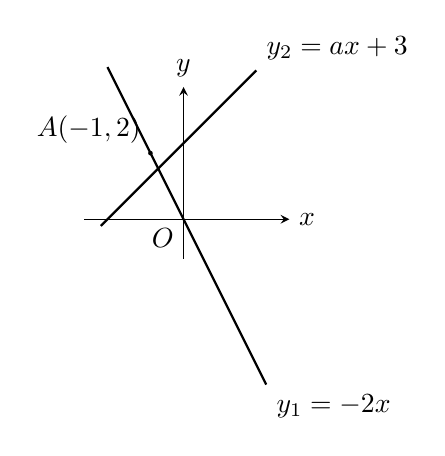
\begin{tikzpicture}[scale=0.42,>=stealth]
  \draw[->] (-3,0)--(3.2,0) node[right] {$x$};
  \draw[->] (0,-1.2)--(0,4) node[above] {$y$};
  \draw[thick] (-2.3,4.6)--(2.5,-5) node[below right] {$y_1=-2x$};
  \draw[thick] (-2.5,-0.2)--(2.2,4.5) node[above right] {$y_2=ax+3$};
  \fill (-1,2) circle (2pt) node[above left] {$A(-1,2)$};
  \node[below left] at (0,0) {$O$};
\end{tikzpicture}
}
  \end{answerareawithdiagramtikz}
  \setcounter{solstep}{0}
  \begin{solutionblock}
    \textbf{答案：}$x>-1$\par\medskip
    \solstep{图像判断}{利用两条直线交点判断函数大小关系。}
  \end{solutionblock}
\end{problem}



\begin{question}[points=4]
  已知直线 $y=kx+b\ (k>0)$ 经过点 $(-2,0)$，那么不等式 $kx+b>0$ 的解集是（\qquad）。
  \paren[$x>-2$]
  \begin{solutionblock}
    由一次函数零点和增减性直接判断。
  \end{solutionblock}
\end{question}



\begin{question}[points=4]
  与直线 $y=3x-1$ 平行且在 $y$ 轴上的截距为 $2$ 的直线一定不经过第（\qquad）象限。
  \paren[第三象限]
  \begin{solutionblock}
    确定直线解析式后判断经过象限。
  \end{solutionblock}
\end{question}



\begin{question}[points=4]
  已知函数 $y=\dfrac23x+1$，如果函数值 $y>5$，那么相应的自变量 $x$ 的取值范围是（\qquad）。
  \paren[$x>6$]
  \begin{solutionblock}
    代入不等式求解即可。
  \end{solutionblock}
\end{question}



\begin{question}[points=4]
  若一次函数 $y=2x+k+4$ 的图象在 $y$ 轴上的截距是 $5$，则 $k=$（\qquad）。
  \paren[$1$]
  \begin{solutionblock}
    直接由常数项等于截距求参数。
  \end{solutionblock}
\end{question}



\begin{question}[points=4]
  当 $m=$（\qquad）时，函数 $y=(2-m)x+m^2-4$（$m$ 是常数）是正比例函数。
  \paren[$-2$]
  \begin{solutionblock}
    令常数项为 0 且一次项系数不为 0。
  \end{solutionblock}
\end{question}



\begin{question}[points=4]
  已知一次函数 $y=kx+k-1$（其中 $k$ 为常数且 $k\ne0$）的图象不经过第二象限，则 $k$ 的取值范围是（\qquad）。
  \paren[$0<k\le1$]
  \begin{solutionblock}
    不过第二象限要求斜率为正且纵截距不大于 $0$，即 $k>0$ 且 $k-1\le0$。
  \end{solutionblock}
\end{question}



\begin{question}[points=4]
  已知一次函数 $y=(2m-2)x+m+1$ 中，$y$ 随 $x$ 的增大而减小，且其图象与 $y$ 轴交点在 $x$ 轴上方，求 $m$ 的取值范围（\qquad）。
  \paren[$-1<m<1$]
  \begin{solutionblock}
    由 $2m-2<0$ 得 $m<1$；由 $m+1>0$ 得 $m>-1$。
  \end{solutionblock}
\end{question}



\begin{question}[points=4]
  我们把直角坐标平面内到 $x$ 轴和到 $y$ 轴距离相等的点称为“特殊点”，那么一次函数 $y=-2x+4$ 的图象上的“特殊点”坐标为（\qquad）。
  \paren[$(1,2)$]
  \begin{solutionblock}
    需理解题目定义的“特殊点”并代入一次函数图像。
  \end{solutionblock}
\end{question}



\begin{question}[points=4]
  秤的应用方便了人们的生活。实验时，若秤杆上秤砣到支点的水平距离为 $x$（厘米）时，对应的物体质量 $y$（斤）可看作 $x$ 的一次函数。表中有若干次实验数据：$x$ 为 $1,3,4,6$，$y$ 为 $0.8,1.2,1.6,1.8$。求当 $x=12$ 厘米时，对应的物体质量 $y$ 为（\qquad）斤。
  \paren[$3$]
  \begin{solutionblock}
    由表格数据识别函数关系并进行预测。
  \end{solutionblock}
\end{question}



\begin{question}[points=4]
  定义：如果直线 $y_1=k_1x+b_1\ (k_1\ne0)$ 与直线 $y_2=k_2x+b_2\ (k_2\ne0)$ 满足 $k_1k_2=-1$ 且 $b_1+b_2=0$，那么称这两条直线具有“和谐关系”。例如，直线 $y_1=2x+3$ 与直线 $y_2=-\dfrac12x-3$ 具有“和谐关系”。如果直线 $y_1=hx+2\ (h>0)$ 与直线 $y_2=kx-2$ 具有“和谐关系”，且这两条直线与 $y$ 轴围成的三角形面积为 $\dfrac{16}{5}$，则 $h=$（\qquad）。
  \paren[$h=\dfrac12$ 或 $h=2$]
  \begin{solutionblock}
    由和谐关系得 $k=-1/h$。两直线与 $y$ 轴截距为 $2$ 和 $-2$，底为 $4$；面积 $16/5$ 得交点到 $y$ 轴距离为 $8/5$，解 $4h/(h^2+1)=8/5$。
  \end{solutionblock}
\end{question}



\begin{question}[points=4]
  在平面直角坐标系 $xOy$ 中，若一次函数 $y=kx+2k+3\ (k\ne0)$ 对于除 $0$ 之外的任意实数 $k$，其图象都经过一个定点 $A$，点 $A'$ 与点 $A$ 关于 $x$ 轴对称，则 $\triangle OAA'$ 的面积为（\qquad）。
  \paren[$6$]
  \begin{solutionblock}
    整理为 $y=k(x+2)+3$，恒过 $A(-2,3)$。关于 $x$ 轴对称得 $A'(-2,-3)$，面积为 $6$。
  \end{solutionblock}
\end{question}



\begin{question}[points=4]
  若一元二次方程 $x^2-5x+a=0$ 无实数根，则一次函数 $y=(a-5)x+a$ 的图象不经过第（\qquad）象限。
  \paren[第四象限]
  \begin{solutionblock}
    无实根得 $a>25/4$，所以斜率 $a-5>0$、截距 $a>0$，图象不经过第四象限。
  \end{solutionblock}
\end{question}


\needspace{8\baselineskip}

\begin{problem}[points=6]
    已知一次函数 $y_1=kx+b$ 与 $y_2=x+a$ 的图象如图所示，有下列结论：① $a<0$；② $b>0$；③ 关于 $x$ 的方程 $kx+b=x+a$ 的解为 $x=3$；④ 当 $x\le3$ 时，$y_2\ge y_1$。其中正确的结论有（\qquad）个。
  \begin{answerareawithdiagramtikz}{28mm}{70mm}{两条一次函数图象}
  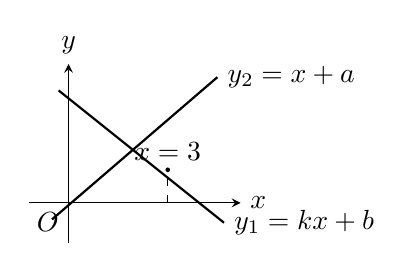
\begin{tikzpicture}[scale=0.42,>=stealth]
  \draw[->] (-1.2,0)--(5.2,0) node[right] {$x$};
  \draw[->] (0,-1.2)--(0,4.2) node[above] {$y$};
  \draw[thick] (-0.3,3.4)--(4.7,-0.6) node[right] {$y_1=kx+b$};
  \draw[thick] (-0.5,-0.5)--(4.5,3.8) node[right] {$y_2=x+a$};
  \fill (3,1.0) circle (2pt) node[above] {$x=3$};
  \draw[dashed] (3,0)--(3,1.0);
  \node[below left] at (0,0) {$O$};
\end{tikzpicture}
}
  \end{answerareawithdiagramtikz}
  \setcounter{solstep}{0}
  \begin{solutionblock}
    \textbf{答案：}$3$\par\medskip
    \solstep{图像判断}{从图像读交点横坐标、两条直线截距和左右位置关系，四个结论中有 $3$ 个正确。}
  \end{solutionblock}
\end{problem}


\section*{二、选择题}


\needspace{14\baselineskip}
\begin{question}[points=4]
  \noindent
  \begin{minipage}[t]{\dimexpr\linewidth-50mm-6mm\relax}
    \vspace{0pt}
    若一次函数 $y=kx+b$ 的图象如图所示，则下列结论中正确的是（\quad）。
    \par
    \begin{choices}[columns=1]
      \item $k<0$
      \item 当 $x=2$ 时，$y=0$
      \item $y$ 随 $x$ 的增大而减小
      \item 当 $x>0$ 时，$y>0$
    \end{choices}
  \end{minipage}\hfill
  \begin{diagramcoltikz}{50mm}{一次函数图象}
  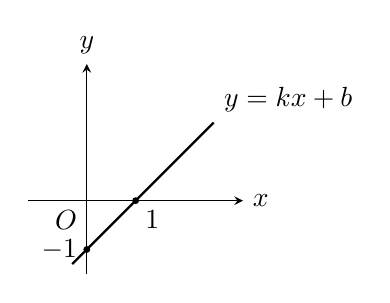
\begin{tikzpicture}[scale=0.62,>=stealth]
  \draw[->] (-1.2,0)--(3.2,0) node[right] {$x$};
  \draw[->] (0,-1.5)--(0,2.8) node[above] {$y$};
  \draw[thick] (-0.3,-1.3)--(2.6,1.6) node[above right] {$y=kx+b$};
  \fill (1,0) circle (2pt) node[below right] {$1$};
  \fill (0,-1) circle (2pt) node[left] {$-1$};
  \node[below left] at (0,0) {$O$};
\end{tikzpicture}
}
  \end{diagramcoltikz}
  \paren[B]
  \begin{solutionblock}
    依据图像判断斜率、截距、零点和函数值符号。
  \end{solutionblock}
\end{question}



\section*{三、解答题}

\needspace{8\baselineskip}

\begin{problem}[points=10]
    在平面直角坐标系中，已知直线 $y_1=-x+3$ 分别交 $x$ 轴、$y$ 轴于 $A,B$ 两点（如图），直线 $y_2=ax+b\ (a>0)$ 交 $x$ 轴于点 $C$。
\begin{enumerate}[label=(\arabic*)]
  \item 求点 $A,B$ 的坐标，并求出直线 $y_2$ 位于 $x$ 轴上方所有点的横坐标取值范围。
  \item 现将直线 $y_2$ 平移，使其经过点 $B$，交 $x$ 轴于点 $D$，如果 $BD=BA$，求 $a$ 的值。
\end{enumerate}
  \begin{answerareawithdiagramtikz}{48mm}{55mm}{坐标轴交点示意}
  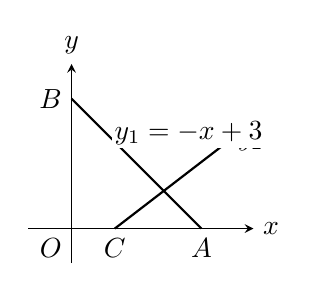
\begin{tikzpicture}[scale=0.55,>=stealth]
  \draw[->] (-1,0)--(4.2,0) node[right] {$x$};
  \draw[->] (0,-0.8)--(0,3.8) node[above] {$y$};
  \draw[thick] (0,3)--(3,0) node[below] {$A$};
  \node[left] at (0,3) {$B$};
  \node[below left] at (0,0) {$O$};
  \draw[thick] (1,0)--(3.6,2.0) node[right] {$y_2$};
  \node[below] at (1,0) {$C$};
  \node[fill=white,inner sep=1pt] at (2.7,2.2) {$y_1=-x+3$};
\end{tikzpicture}
}
  \end{answerareawithdiagramtikz}
  \setcounter{solstep}{0}
  \begin{solutionblock}
    \textbf{答案：}(1) $A(3,0)$，$B(0,3)$，$x>-1$；(2) $a=1$。\par\medskip
    \solstep{读题建模}{综合坐标轴交点、函数正负区间、平移后斜率参数。}
    \solstep{计算与判断}{按题目给出的函数、坐标或表格条件列式求解，最后回代检查。}
  \end{solutionblock}
\end{problem}


\needspace{8\baselineskip}

\begin{problem}[points=10]
    某地区交通管理部门通过对道路流量的大数据分析可知，某东西路上车辆的平均速度 $y$（千米/时）与该条路上每百米车的数量 $x$（辆）的关系如图所示。
\begin{enumerate}[label=(\arabic*)]
  \item 求 $y$ 关于 $x$ 的函数解析式（不必写 $x$ 的取值范围）。
  \item 如果某时刻监测到这一东西路上车辆的平均速度为 $30$ 千米/时，求此时这条路上每百米车的数量。
  \item 如果车辆的平均速度小于 $20$ 千米/时，将严重拥堵，需启动限流措施；若此时开始这一路段上每百米车的数量以每 $4$ 分钟增加 $1$ 辆，为避免严重拥堵，求约几分钟后需启动限流措施。
\end{enumerate}
  \begin{answerareawithdiagramtikz}{48mm}{60mm}{速度与车辆数关系图}
  \begin{tikzpicture}[scale=0.065,>=stealth]
  \draw[->] (0,0)--(45,0) node[right] {$x$（辆）};
  \draw[->] (0,0)--(0,75) node[above] {$y$（千米/时）};
  \draw[thick] (5,70)--(25,30);
  \draw[dashed] (10,0)--(10,60)--(0,60);
  \draw[dashed] (20,0)--(20,40)--(0,40);
  \node[below] at (10,0) {$10$}; \node[below] at (20,0) {$20$};
  \node[left] at (0,60) {$60$}; \node[left] at (0,40) {$40$};
  \node[below left] at (0,0) {$O$};
\end{tikzpicture}
}
  \end{answerareawithdiagramtikz}
  \setcounter{solstep}{0}
  \begin{solutionblock}
    \textbf{答案：}(1) $y=-2x+80$；(2) $25$ 辆；(3) 约 $20$ 分钟后。\par\medskip
    \solstep{读题建模}{从图像建立一次函数模型，并用不等式判断实际情境。}
    \solstep{计算与判断}{按题目给出的函数、坐标或表格条件列式求解，最后回代检查。}
  \end{solutionblock}
\end{problem}


\needspace{8\baselineskip}

\begin{problem}[points=10]
    已知，如图，点 $A$ 的坐标为 $(0,4)$，点 $B$ 在反比例函数 $y=-\dfrac8x$ 的图象上。
\begin{enumerate}[label=(\arabic*)]
  \item 当 $\triangle AOB$ 的面积为 $12$ 时，求点 $B$ 的坐标。
  \item 点 $C$ 在 $y$ 轴负半轴，点 $D$ 在线段 $BO$ 的延长线上，当四边形 $ABCD$ 为矩形时，求直线 $AB$ 的解析式。
\end{enumerate}
  \begin{answerareawithdiagramtikz}{48mm}{58mm}{反比例函数与点 A、B}
  \begin{tikzpicture}[scale=0.52,>=stealth]
  \draw[->] (-0.8,0)--(7,0) node[right] {$x$};
  \draw[->] (0,-2.5)--(0,4.8) node[above] {$y$};
  \draw[domain=1.9:6.8,smooth,variable=\x,thick] plot ({\x},{-8/\x});
  \fill (0,4) circle (2pt) node[left] {$A(0,4)$};
  \fill (6,-1.333) circle (2pt) node[below] {$B$};
  \draw[thick] (0,4)--(6,-1.333);
  \node[below left] at (0,0) {$O$};
  \node[right] at (5.2,-2.0) {$y=-\frac{8}{x}$};
\end{tikzpicture}
}
  \end{answerareawithdiagramtikz}
  \setcounter{solstep}{0}
  \begin{solutionblock}
    \textbf{答案：}(1) $B(6,-\dfrac43)$；(2) $y=-\dfrac89x+4$。\par\medskip
    \solstep{读题建模}{综合反比例函数点坐标、面积关系、矩形性质和直线解析式。}
    \solstep{计算与判断}{按题目给出的函数、坐标或表格条件列式求解，最后回代检查。}
  \end{solutionblock}
\end{problem}


\needspace{8\baselineskip}

\begin{problem}[points=10]
    如图，一次函数 $y=2x+4$ 的图象与 $x$ 轴、$y$ 轴分别交于 $A,B$ 两点，与反比例函数 $y=\dfrac{k}{x}\ (k\ne0,x>0)$ 的图象交于点 $C$，过点 $B$ 作 $x$ 轴的平行线与该反比例函数的图象交于点 $D$，连接 $CD$。
\begin{enumerate}[label=(\arabic*)]
  \item 求 $A,B$ 两点的坐标。
  \item 如果 $BC=DC$，求 $k$ 的值。
\end{enumerate}
  \begin{answerareawithdiagramtikz}{48mm}{58mm}{一次函数与反比例函数}
  \begin{tikzpicture}[scale=0.46,>=stealth]
  \draw[->] (-3,0)--(6,0) node[right] {$x$};
  \draw[->] (0,-0.8)--(0,6) node[above] {$y$};
  \draw[thick] (-2,0)--(1,6);
  \node[fill=white,inner sep=1pt] at (-1.0,5.3) {$y=2x+4$};
  \draw[domain=1.2:5.8,smooth,variable=\x,thick] plot ({\x},{16/\x});
  \draw[dashed] (0,4)--(4,4);
  \fill (-2,0) circle (2pt) node[below] {$A$};
  \fill (0,4) circle (2pt) node[left] {$B$};
  \fill (4,4) circle (2pt) node[above right] {$D$};
  \node[below left] at (0,0) {$O$};
  \node[right] at (4.5,3.0) {$y=\frac{k}{x}$};
\end{tikzpicture}
}
  \end{answerareawithdiagramtikz}
  \setcounter{solstep}{0}
  \begin{solutionblock}
    \textbf{答案：}(1) $A(-2,0)$，$B(0,4)$；(2) $k=16$。\par\medskip
    \solstep{读题建模}{需要读图建立交点坐标，再用线段相等求反比例函数参数。}
    \solstep{计算与判断}{按题目给出的函数、坐标或表格条件列式求解，最后回代检查。}
  \end{solutionblock}
\end{problem}


\needspace{8\baselineskip}

\begin{problem}[points=10]
    如图，为某公园“水上滑梯”的侧面图，其中 $BC$ 段可看成是一段双曲线。建立如图所示的坐标系后，矩形 $AOBE$ 为向上攀爬的梯子，$OA=6$ 米，进口 $AB\parallel OD$，且 $AB=2$ 米，出口 $C$ 点距水面的距离为 $CD$。
\begin{enumerate}[label=(\arabic*)]
  \item 求 $BC$ 段滑梯所在双曲线的表达式（$x\ge2$）。
  \item 若 $CD$ 为 $1.5$ 米，求 $B,C$ 之间的水平距离 $DE$ 的长度。
\end{enumerate}
  \begin{answerareawithdiagramtikz}{48mm}{58mm}{水上滑梯侧面示意}
  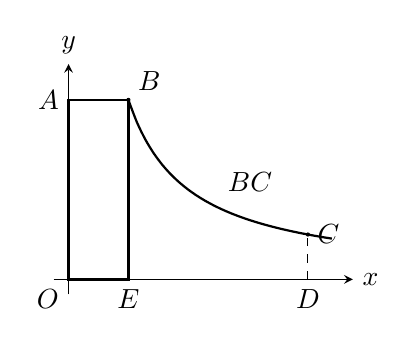
\begin{tikzpicture}[scale=0.38,>=stealth]
  \draw[->] (-0.5,0)--(9.5,0) node[right] {$x$};
  \draw[->] (0,-0.5)--(0,7.2) node[above] {$y$};
  \draw[thick] (0,0)--(0,6)--(2,6)--(2,0)--cycle;
  \draw[domain=2:8.8,smooth,variable=\x,thick] plot ({\x},{12/\x});
  \draw[dashed] (8,0)--(8,1.5);
  \fill (2,6) circle (2pt) node[above right] {$B$};
  \fill (8,1.5) circle (2pt) node[right] {$C$};
  \node[left] at (0,6) {$A$}; \node[below left] at (0,0) {$O$};
  \node[below] at (2,0) {$E$}; \node[below] at (8,0) {$D$};
  \node[above right] at (5,2.6) {$BC$};
\end{tikzpicture}
}
  \end{answerareawithdiagramtikz}
  \setcounter{solstep}{0}
  \begin{solutionblock}
    \textbf{答案：}(1) $y=\dfrac{12}{x}$；(2) $DE=6$ 米。\par\medskip
    \solstep{读题建模}{需要根据实际图形读点坐标，建立反比例函数模型并求水平距离。}
    \solstep{计算与判断}{按题目给出的函数、坐标或表格条件列式求解，最后回代检查。}
  \end{solutionblock}
\end{problem}


\clearpage
\section*{参考答案}


\begin{keyideabox}
  \textbf{答案汇总}
  填空题第1题：$x>2$

填空题第2题：$y=-3x-6$

填空题第3题：$y=x-5$

填空题第4题：$x=1,y=2$

填空题第5题：$y=5x-3\sqrt3+5$

填空题第6题：$5$

填空题第7题：$x>-1$

填空题第8题：$x>-2$

填空题第9题：第三象限

填空题第10题：$x>6$

填空题第11题：$1$

填空题第12题：$-2$

填空题第13题：$0<k\le1$

填空题第14题：$-1<m<1$

填空题第15题：$(1,2)$

填空题第16题：$3$

填空题第17题：$h=\dfrac12$ 或 $h=2$

填空题第18题：$6$

填空题第19题：第四象限

填空题第20题：$3$

选择题第1题：B

解答题第1题：(1) $A(3,0)$，$B(0,3)$，$x>-1$；(2) $a=1$。

解答题第2题：(1) $y=-2x+80$；(2) $25$ 辆；(3) 约 $20$ 分钟后。

解答题第3题：(1) $B(6,-\dfrac43)$；(2) $y=-\dfrac89x+4$。

解答题第4题：(1) $A(-2,0)$，$B(0,4)$；(2) $k=16$。

解答题第5题：(1) $y=\dfrac{12}{x}$；(2) $DE=6$ 米。
\end{keyideabox}



\end{document}
